\documentclass{article}
\usepackage{xeCJK}
\usepackage{amsmath}
\usepackage{geometry}
\usepackage{graphicx}


\setCJKmainfont{Microsoft YaHei}
\linespread{1.5}
\setlength{\parindent}{0pt}
\geometry{a4paper,scale=0.75}

\begin{document}
一.\\
(1)编译器总体结构如下: \\
\begin{figure}[htbp]
    \centering
    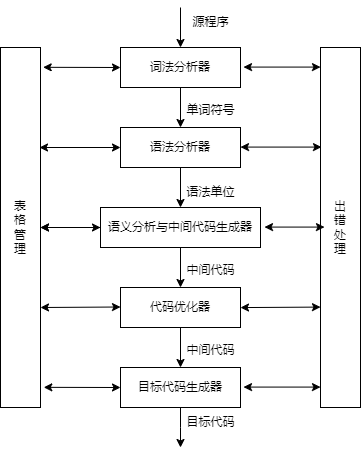
\includegraphics[scale=0.5]{complier.png}
    \caption{编译器结构}
\end{figure}
\\
(i)词法分析器将源代码的字符流转化为一系列词法单元(token),这些单元通常代表最小的语法元素,如关键词、运算符、标识符等,
同时去除无用的空白符、注释,并报告词法错误。\\
(ii)语法分析器根据词法单元(token)的顺序检查源代码的语法结构,生成抽象语法树(AST)。
其目的是确保源代码符合语言的语法规则,并捕捉语法错误。\\
(iii)语义分析器会对AST进行语义检查,确保每个操作符、变量和函数调用的使用方式正确。
中间代码生成器则将经过语义检查的代码转换为中间表示,这种表示比源代码更接近机器代码。\\
(iv)代码优化器通过分析和改进中间代码,去除冗余操作,提高执行效率。\\
(v)目标代码生成器将优化后的中间代码转换为特定硬件平台的机器代码或汇编代码。同时负责寄存器分配、指令选择和指令排布等任务。\\
(vi)表格管理模块负责管理编译过程中所需的符号表、类型表、常量表等信息,这些表格用于存储变量、函数和数据类型等信息。\\
(vii)出错处理模块负责在编译过程中处理各种错误(如词法错误、语法错误、语义错误等),并向用户报告有用的错误信息。\\
\\
(2)$T$型图如下: \\
\begin{figure}[htbp]
    \centering
    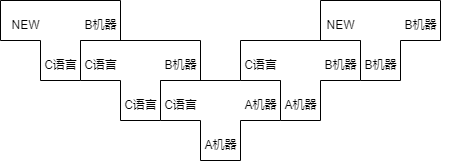
\includegraphics[scale=0.6]{t.png}
    \caption{t型图}
\end{figure}
\newpage
二.\\
(1)
对于 $id + id * (id - id)$, \\
最左推导:
\begin{align*}
    E & \Rightarrow E + T \Rightarrow T + T \Rightarrow F + T \Rightarrow P + T \Rightarrow id + T \Rightarrow id + T * F\\
      & \Rightarrow id + F * F \Rightarrow id + P * F \Rightarrow id + id * F  \Rightarrow id + id * P\\
      & \Rightarrow id + id * (E) \Rightarrow id + id * (E - T) \Rightarrow id + id * (T - T)  \\
      & \Rightarrow id + id * (F - T) \Rightarrow id + id * (P - T) \Rightarrow id + id * (id - T)  \\
      & \Rightarrow id + id * (id - F) \Rightarrow id + id * (id - P) \Rightarrow id + id * (id - id)
\end{align*}
最右推导:
\begin{align*}
    E & \Rightarrow E + T \Rightarrow E + T * F \Rightarrow E + T * P \Rightarrow E + T * (E)  \\
      & \Rightarrow E + T * (E - T) \Rightarrow E + T * (E - F) \Rightarrow E + T * (E - P)  \\
      & \Rightarrow E + T * (E - id) \Rightarrow E + T * (T - id) \Rightarrow E + T * (F - id)  \\
      & \Rightarrow E + T * (P - id) \Rightarrow E + T * (id - id) \Rightarrow E + F * (id - id)  \\
      & \Rightarrow E + P * (id - id) \Rightarrow E + id * (id - id) \Rightarrow T + id * (id - id)  \\
      & \Rightarrow F + id * (id - id) \Rightarrow P + id * (id - id) \Rightarrow id + id * (id - id)
\end{align*}
任意推导:
\begin{align*}
    E & \Rightarrow E + T \Rightarrow T + T \Rightarrow F + T \Rightarrow P + T \Rightarrow id + T \Rightarrow id + T * F\\
      & \Rightarrow id + F * F \Rightarrow id + P * F \Rightarrow id + id * F \Rightarrow id + id * P \\
      & \Rightarrow id + id * (E) \Rightarrow id + id * (E - T) \Rightarrow id + id * (E - F)  \\
      & \Rightarrow id + id * (T - F) \Rightarrow id + id * (F - F) \Rightarrow id + id * (P - F)  \\
      & \Rightarrow id + id * (id - F) \Rightarrow id + id * (id - P) \Rightarrow id + id * (id - id)
\end{align*}
\\
对于$(c + id) * (id + c)$, \\
最左推导:
\begin{align*}
    E & \Rightarrow T \Rightarrow T * F \Rightarrow F * F \Rightarrow P * F \Rightarrow (E) * F \Rightarrow (E + T) * F\\
      & \Rightarrow (T + T) * F \Rightarrow (F + T) * F \Rightarrow (P + T) * F \Rightarrow (c + T) * F\\
      & \Rightarrow (c + F) * F \Rightarrow (c + P) * F \Rightarrow (c + id) * F \Rightarrow (c + id) * P\\
      & \Rightarrow (c + id) * (E) \Rightarrow (c + id) * (E + T) \Rightarrow (c + id) * (T + T)\\
      & \Rightarrow (c + id) * (F + T) \Rightarrow (c + id) * (P + T) \Rightarrow (c + id) * (id + T)\\
      & \Rightarrow (c + id) * (id + F) \Rightarrow (c + id) * (id + P) \Rightarrow (c + id) * (id + c)   
\end{align*}
最右推导:
\begin{align*}
    E & \Rightarrow T \Rightarrow T * F \Rightarrow T * P \Rightarrow T * (E) \Rightarrow T * (E + T) \Rightarrow T * (E + F)\\
      & \Rightarrow T * (E + P) \Rightarrow T * (E + c) \Rightarrow T * (T + c) \Rightarrow T * (F + c) \\
      & \Rightarrow T * (P + c) \Rightarrow T * (id + c) \Rightarrow F * (id + c) \Rightarrow P * (id + c) \\
      & \Rightarrow (E) * (id + c) \Rightarrow (E + T) * (id + c) \Rightarrow (E + F) * (id + c) \\
      & \Rightarrow (E + P) * (id + c) \Rightarrow (E + id) * (id + c) \Rightarrow (T + id) * (id + c) \\
      & \Rightarrow (F + id) * (id + c) \Rightarrow (P + id) * (id + c) \Rightarrow (c + id) * (id + c)
\end{align*}
任意推导:
\begin{align*}
    E & \Rightarrow T \Rightarrow T * F \Rightarrow F * F \Rightarrow P * F \Rightarrow (E) * F \Rightarrow (E + T) * F\\
      & \Rightarrow (T + T) * F \Rightarrow (F + T) * F \Rightarrow (P + T) * F \Rightarrow (P + F) * F\\
      & \Rightarrow (c + F) * F \Rightarrow (c + P) * F \Rightarrow (c + id) * F \Rightarrow (c + id) * P\\
      & \Rightarrow (c + id) * (E) \Rightarrow (c + id) * (E + T) \Rightarrow (c + id) * (T + T)\\
      & \Rightarrow (c + id) * (F + T) \Rightarrow (c + id) * (P + T) \Rightarrow (c + id) * (id + T)\\
      & \Rightarrow (c + id) * (id + F) \Rightarrow (c + id) * (id + P) \Rightarrow (c + id) * (id + c)    
\end{align*}
(2)
对于 $id + id * (id - id)$, \\
最右归约:
\begin{align*}
    (c + id) * (id + c) & \Leftarrow (c + id) * (id + P) \Leftarrow (c + id) * (id + F) \\
                        & \Leftarrow (c + id) * (id + T) \Leftarrow (c + id) * (P + T) \\
                        & \Leftarrow (c + id) * (F + T) \Leftarrow (c + id) * (T + T) \\
                        & \Leftarrow (c + id) * (E + T) \Leftarrow (c + id) * (E) \\
                        & \Leftarrow (c + id) * P \Leftarrow (c + id) * F \\
                        & \Leftarrow (c + P) * F \Leftarrow (c + F) * F \\
                        & \Leftarrow (c + T) * F \Leftarrow (P + T) * F \\
                        & \Leftarrow (F + T) * F \Leftarrow (T + T) * F \\
                        & \Leftarrow (E + T) * F \Leftarrow (E) * F \\
                        & \Leftarrow P * F \Leftarrow F * F \\
                        & \Leftarrow T * F \Leftarrow T \Leftarrow E
\end{align*}

最左规约:
\begin{align*}
    id + id * (id - id) & \Leftarrow P + id * (id - id) \Leftarrow F + id * (id - id) \\
                        & \Leftarrow T + id * (id - id) \Leftarrow E + id * (id - id) \\
                        & \Leftarrow E + P * (id - id) \Leftarrow E + F * (id - id) \\
                        & \Leftarrow E + T * (id - id) \Leftarrow E + T * (P - id) \\
                        & \Leftarrow E + T * (F - id) \Leftarrow E + T * (E - id) \\
                        & \Leftarrow E + T * (E - P) \Leftarrow E + T * (E - F) \\
                        & \Leftarrow E + T * (E) \Leftarrow E + T * F \\
                        & \Leftarrow E + T \Leftarrow E
\end{align*}

上述任意推导对应的规约:
\begin{align*}
    id + id * (id - id) & \Leftarrow id + id * (id - P) \Leftarrow id + id * (id - F) \\
                        & \Leftarrow id + id * (F - F) \Leftarrow id + id * (T - F) \\
                        & \Leftarrow id + id * (E - F) \Leftarrow id + id * (E - T) \\
                        & \Leftarrow id + id * (E) \Leftarrow id + id * P \\
                        & \Leftarrow id + id * F \Leftarrow id + F * F \\
                        & \Leftarrow id + T * F \Leftarrow id + T \\
                        & \Leftarrow P + T \Leftarrow F + T \\
                        & \Leftarrow T + T \Leftarrow E + T \\
                        & \Leftarrow E
\end{align*}

对于$(c + id) * (id + c)$, \\
最右规约:
\begin{align*}
    (c + id) * (id + c) & \Leftarrow (c + id) * (id + P) \Leftarrow (c + id) * (id + F) \\
                        & \Leftarrow (c + id) * (id + T) \Leftarrow (c + id) * (P + T) \\
                        & \Leftarrow (c + id) * (F + T) \Leftarrow (c + id) * (T + T) \\
                        & \Leftarrow (c + id) * (E + T) \Leftarrow (c + id) * (E) \\
                        & \Leftarrow (c + id) * P \Leftarrow (c + id) * F \\
                        & \Leftarrow (c + P) * F \Leftarrow (c + F) * F \\
                        & \Leftarrow (c + T) * F \Leftarrow (P + T) * F \\
                        & \Leftarrow (F + T) * F \Leftarrow (T + T) * F \\
                        & \Leftarrow (E + T) * F \Leftarrow (E) * F \\
                        & \Leftarrow P * F \Leftarrow F * F \\
                        & \Leftarrow T * F \Leftarrow T \Leftarrow E
\end{align*}
最左规约:
\begin{align*}
    (c + id) * (id + c) & \Leftarrow (P + id) * (id + c) \Leftarrow (F + id) * (id + c) \\
                        & \Leftarrow (T + id) * (id + c) \Leftarrow (E + id) * (id + c) \\
                        & \Leftarrow (E + P) * (id + c) \Leftarrow (E + F) * (id + c) \\
                        & \Leftarrow (E + T) * (id + c) \Leftarrow (E) * (id + c) \\
                        & \Leftarrow P * (id + c) \Leftarrow F * (id + c) \\
                        & \Leftarrow T * (id + c) \Leftarrow T * (P + c) \\
                        & \Leftarrow T * (F + c) \Leftarrow T * (T + c) \\
                        & \Leftarrow T * (E + c) \Leftarrow T * (E + P) \\
                        & \Leftarrow T * (E + F) \Leftarrow T * (E + T) \\
                        & \Leftarrow T * (E) \Leftarrow T * P \\
                        & \Leftarrow T * F \Leftarrow T \\
                        & \Leftarrow E
\end{align*}

上述任意推导对应的规约:
\begin{align*}
    (c + id) * (id + c) & \Leftarrow (c + id) * (id + P) \Leftarrow (c + id) * (id + F) \\
                        & \Leftarrow (c + id) * (id + T) \Leftarrow (c + id) * (P + T) \\
                        & \Leftarrow (c + id) * (F + T) \Leftarrow (c + id) * (T + T) \\
                        & \Leftarrow (c + id) * (E + T) \Leftarrow (c + id) * (E) \\
                        & \Leftarrow (c + id) * P \Leftarrow (c + id) * F \\
                        & \Leftarrow (c + P) * F \Leftarrow (c + F) * F \\
                        & \Leftarrow (P + F) * F \Leftarrow (P + T) * F \\
                        & \Leftarrow (F + T) * F \Leftarrow (T + T) * F \\
                        & \Leftarrow (E + T) * F \Leftarrow (E) * F \\
                        & \Leftarrow P * F \Leftarrow F * F \\
                        & \Leftarrow T * F \Leftarrow T \\
                        & \Leftarrow E
\end{align*}
\newpage
(3)
$id + id * (id - id)$ 的最左语法树如下: \\
\begin{figure}[htbp]
    \centering
    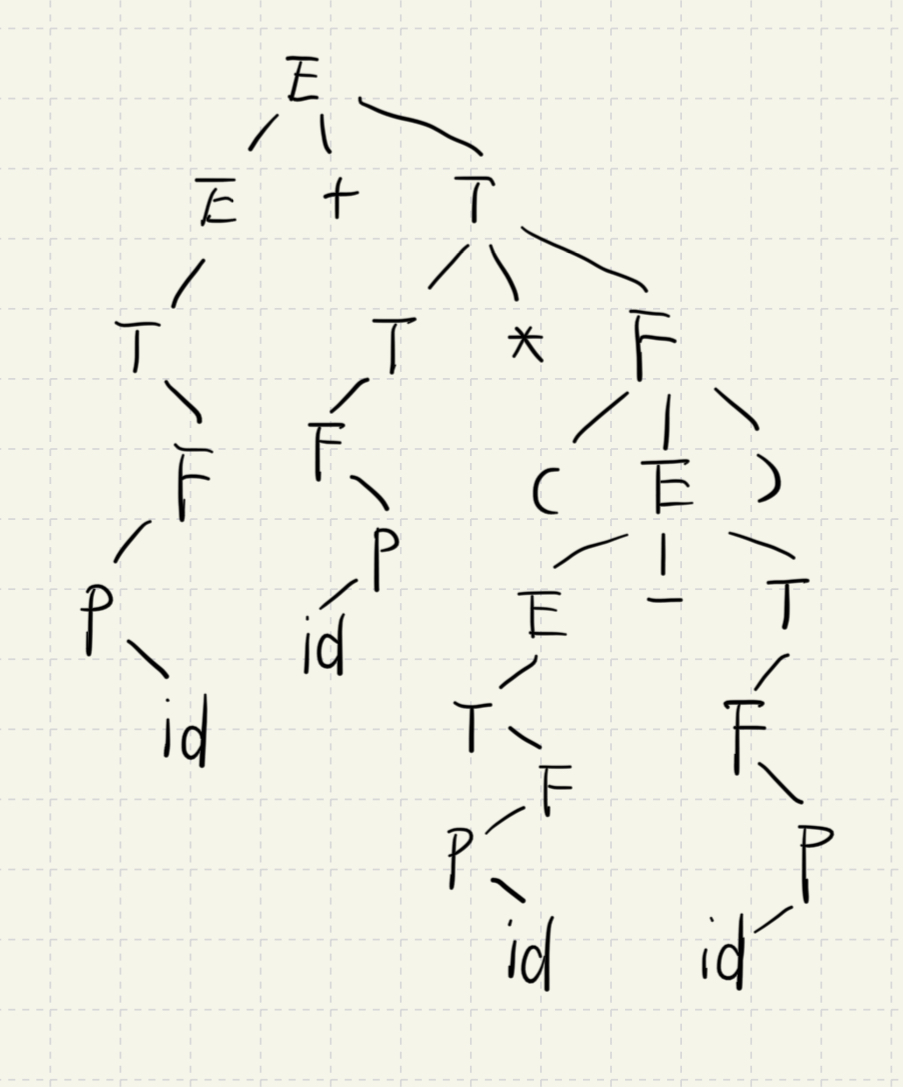
\includegraphics[scale=0.1]{tree1.jpg}
    \caption{语法树1}
\end{figure}
\\
$(c + id) * (id + c)$ 的最左语法树如下: \\
\begin{figure}[htbp]
    \centering
    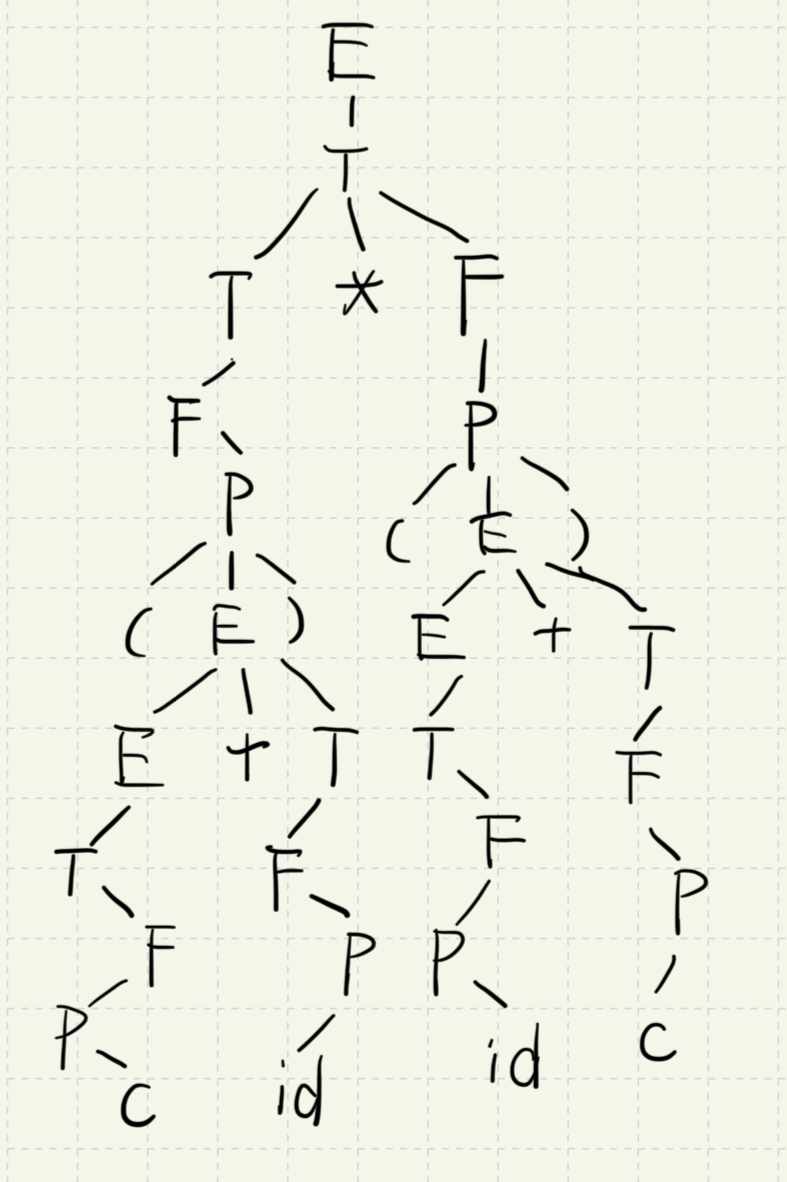
\includegraphics[scale=0.1]{tree2.jpg}
    \caption{语法树2}
\end{figure}
\\
(4)
对于 $id + id * (id - id)$, \\
短语为: $id, id, id, id, id - id, (id - id), id * (id - id), id + id * (id - id)$ \\
简单短语为: $id, id, id, id$ \\
句柄为: $id$ \\
\\
对于 $(c + id) * (id + c)$, \\
短语为: $c, c, id, id, c + id, id + c, (c + id), (id + c), (c + id) * (id + c)$ \\
简单短语为: $c, c, id, id$ \\
句柄为: $c$ \\ 
三.\\
(1)根据文法,列出方程组如下:
\[
\begin{cases}
    \text{<标号说明>} = \text{LABEL} \text{<标号段>} \\
    \text{<标号表>} = d \; \text{<标号段>} \\
    \text{<标号段>} = d \; \text{<标号段>} \\
    \text{<标号段>} = , \; \text{<标号>} \\
    \text{<标号段>} = ; \\
    \text{<标号>} = d \; \text{<标号段>} 
\end{cases}
\]
求解得到正则表达式为
\[
    \text{LABEL}\; d(d|,d)^{*};
\]
(2)上述正则表达式对应的DFA如下: \\
\begin{figure}[htbp]
    \centering
    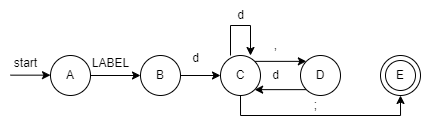
\includegraphics[scale=0.6]{DFA.png}
    \caption{DFA}
\end{figure}
\\
四.\\ 
(1)
\begin{align*}
& S \to bES' \\
& S' \to aES' | \epsilon \\
& F \to S | a \\
& E \to Fc
\end{align*}
(2)
First集合如下:
\begin{align*}
& \text{First}(S) = \{b\} \\
& \text{First}(S') = \{a, \epsilon\} \\
& \text{First}(F) = \{a, b\} \\
& \text{First}(E) = \{a, b\} \\
& \text{First}(a) = \{a\} \\
& \text{First}(b) = \{b\} \\
& \text{First}(c) = \{c\}
\end{align*}
Follow集合如下:
\begin{align*}
& \text{Follow}(S) = \{\#, c\} \\
& \text{Follow}(S') = \{\#, c\} \\
& \text{Follow}(F) = \{c\} \\
& \text{Follow}(E) = \{a, c, \#\}
\end{align*}
(3)
由于
\begin{align*}
& \text{First}(S) \cap \text{First}(a) = \emptyset \\
& \text{Follow}(S') \cap \text{First}(aES') = \emptyset
\end{align*}
故该文法是$LL(1)$文法.
预测分析表如下:
\[
\begin{array}{|l|l|l|l|l|}
     & a & b & c & \#\\
    \hline
    S & & \to bES' & & \\
    \hline
    S' & \to aES' & & \epsilon & \epsilon \\
    \hline
    E & \to Fc & \to Fc & & \\
    \hline
    F & \to a & \to S & &
\end{array}
\]

五. \\ 
(1)
\begin{align*}
    & \text{<var\_list>} \to \text{id} \text{<var\_list>}' \\
    & \text{<var\_list>}' \to \text{,} \text{<var\_list>} | \epsilon
\end{align*}
(2)
First集合如下:
\begin{align*}
& \text{First}(\text{<declaration>}) = \{\text{int}, \text{float}\} \\
& \text{First}(\text{<type>}) = \{\text{int}, \text{float}\} \\
& \text{First}(\text{<var\_list>}) = \{\text{id}\} \\
& \text{First}(\text{<var\_list>}') = \{'\text{,}' \; , \epsilon\} \\
& \text{First}(\text{int}) = \{\text{int}\} \\
& \text{First}(\text{float}) = \{\text{float}\} \\
& \text{First}(\text{id}) = \{\text{id}\} \\
& \text{First}(\text{,}) = \{\text{,}\}
\end{align*}
Follow集合如下:
\begin{align*}
& \text{Follow}(\text{<declaration>}) = \{\# \} \\
& \text{Follow}(\text{<type>}) = \{\text{id}\} \\
& \text{Follow}(\text{<var\_list>}) = \{\# \} \\
& \text{Follow}(\text{<var\_list>}') = \{\# \}
\end{align*}
(3)
由于
\begin{align*}
& \text{First}(\text{int}) \cap \text{First}(\text{float}) = \emptyset \\
& \text{First}(\text{,<var\_list>}) \cap \text{First}(\epsilon) = \emptyset \\
& \text{First}(\text{,<var\_list>}) \cap \text{Follow}(\text{<var\_list>}') = \emptyset 
\end{align*}    
故该文法是$LL(1)$文法. \\
(4)
预测分析表如下:
\[
\begin{array}{|l|l|l|l|l|l|}
     & \text{int} & \text{float} & \text{id} & \text{,} & \#\\
    \hline
    \text{<declaration>} & \to \text{<type><var\_list>} & \to \text{<type><var\_list>} & & & \\
    \hline
    \text{<type>} & \to \text{int} & \to \text{float} & & & \\
    \hline
    \text{<var\_list>} & & & \to \text{id} \text{<var\_list>}' & & \\
    \hline
    \text{<var\_list>}' & & & & \to \text{,<var\_list>} & \to \epsilon
\end{array}
\]
(5)分析过程如下:
\[
\begin{array}{|l|l|l|}
    \text{栈} & \text{输入缓冲} & \text{输出} \\
    \hline
    \text{\#<declaration>} & \text{int x,y,z\#} & \\
    \hline
    \text{\#<var\_list><type>} & \text{int x,y,z\#} & \text{<declaration>} \to \text{<type><var\_list>} \\
    \hline
    \text{\#<var\_list>int} & \text{int x,y,z\#} & \text{<type>} \to \text{int} \\
    \hline
    \text{\#<var\_list>} & \text{x,y,z\#} & \\
    \hline
    \text{\#}\text{<var\_list>}'\text{id} & \text{x,y,z\#} & \text{<var\_list>} \to \text{id} \text{<var\_list>}' \\
    \hline
    \text{\#}\text{<var\_list>}' & \text{,y,z\#} & \\
    \hline
    \text{\#<var\_list>,} & \text{y,z\#} & \text{<var\_list>}' \to \text{,<var\_list>} \\
    \hline
    \text{\#<var\_list>} & \text{y,z\#} & \\
    \hline
    \text{\#}\text{<var\_list>}'\text{id} & \text{y,z\#} & \text{<var\_list>} \to \text{id} \text{<var\_list>}' \\
    \hline
    \text{\#}\text{<var\_list>}' & \text{,z\#} & \\
    \hline
    \text{\#<var\_list>,} & \text{,z\#} & \text{<var\_list>}' \to \text{,<var\_list>} \\
    \hline
    \text{\#<var\_list>} & \text{z\#} & \\
    \hline
    \text{\#}\text{<var\_list>}'\text{id} & \text{z\#} & \text{<var\_list>} \to \text{id} \text{<var\_list>}' \\
    \hline
    \text{\#}\text{<var\_list>}' & \text{\#} & \\
    \hline
    \text{\#} & \text{\#} & \text{<var\_list>}' \to \epsilon 
\end{array}
\]
\end{document}